Johannes Sedlmeir und seine Kollegen haben die Berechnungen mit Werten aus dem Jahr 2020 durchgeführt\citebib{sedlmeir}{S.602}{vgl. }. Allerdings haben sie den PUE nicht berücksichtigt. Wenn wir die in ihrer Arbeit errechneten Werte für den minimalen und maximalen Stromverbrauch mit dem minimalen und maximalen PUE multiplizieren ergibt sich folgendes Diagramm:
\FloatBarrier
\begin{figure}[ht!]
    \centering
    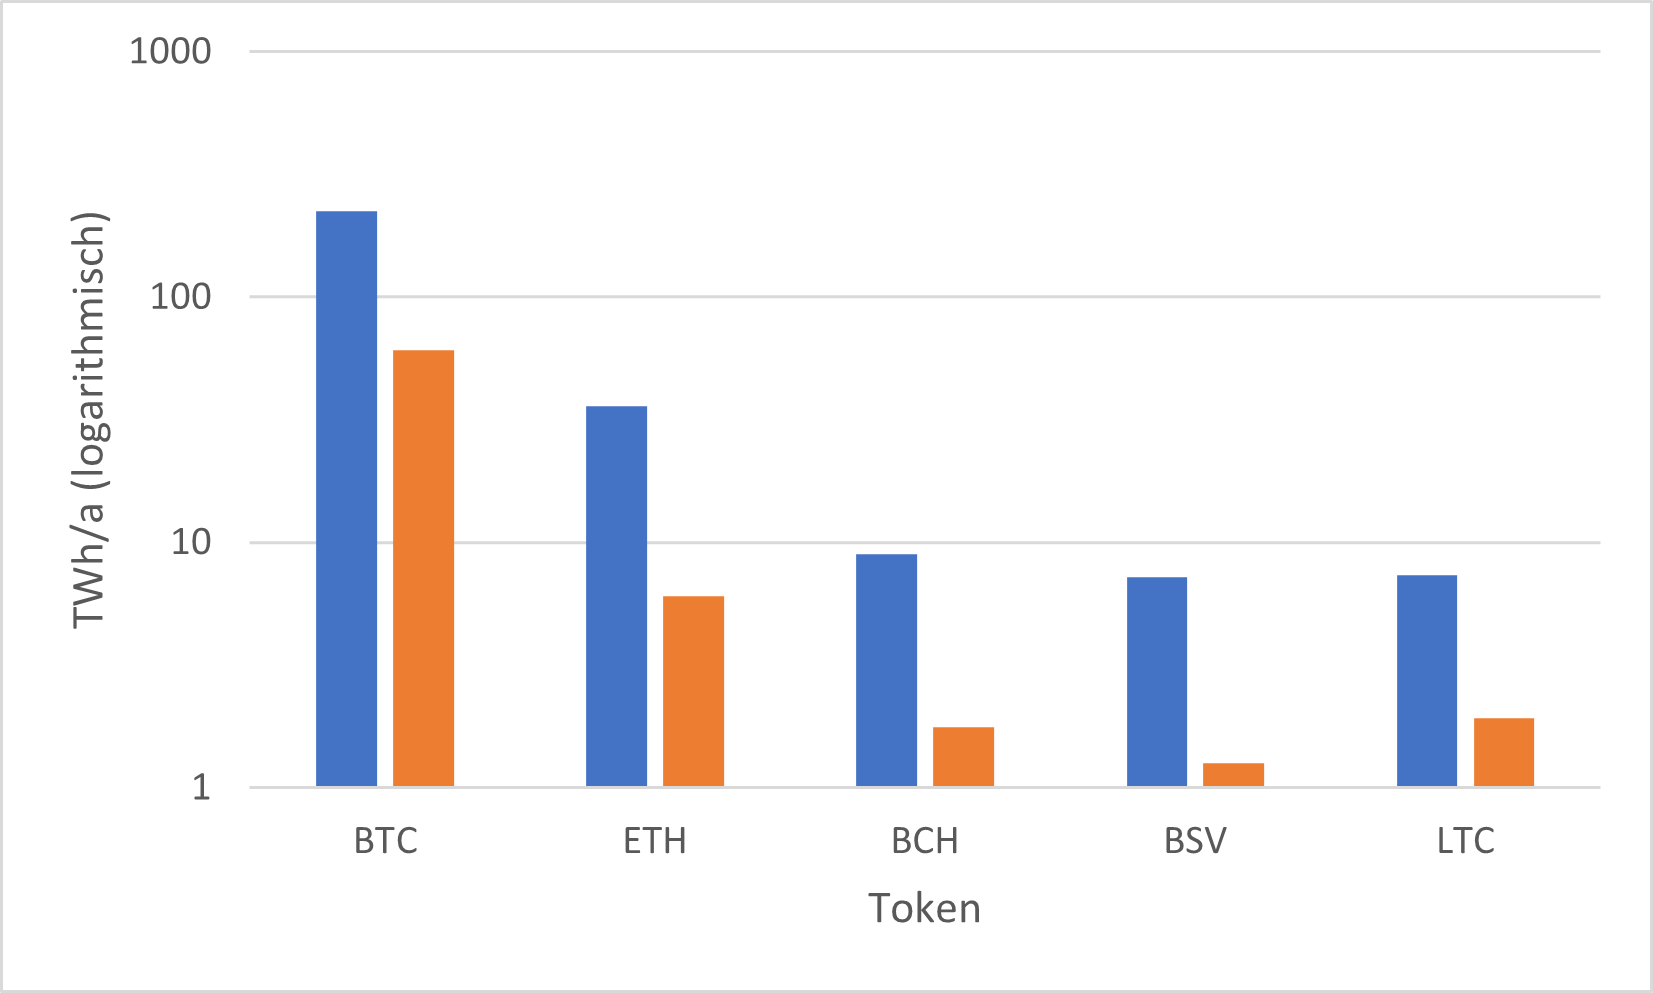
\includegraphics[width=.75\textwidth]{quellen/pow_2020.png}
    \caption{Stromverbrauch von PoW-Netzwerken 2020}
\end{figure}
\FloatBarrier
\clearpage
\noindent Als Vergleichsgröße zur Beliebtheit der Kryptowährungen eignet sich deren Marktkapitalisierung. Diese wird aus dem aktuellen Preis und der Umlaufmenge gebildet\citebib{cmcPoW}{}{vgl. }. Die Marktkapitalisierung der einzelnen Tokens im Jahre 2020 zeigt folgende Verteilung\citebib{sedlmeir}{S.602}{vgl. }:
\FloatBarrier
\begin{figure}[ht!]
    \centering
    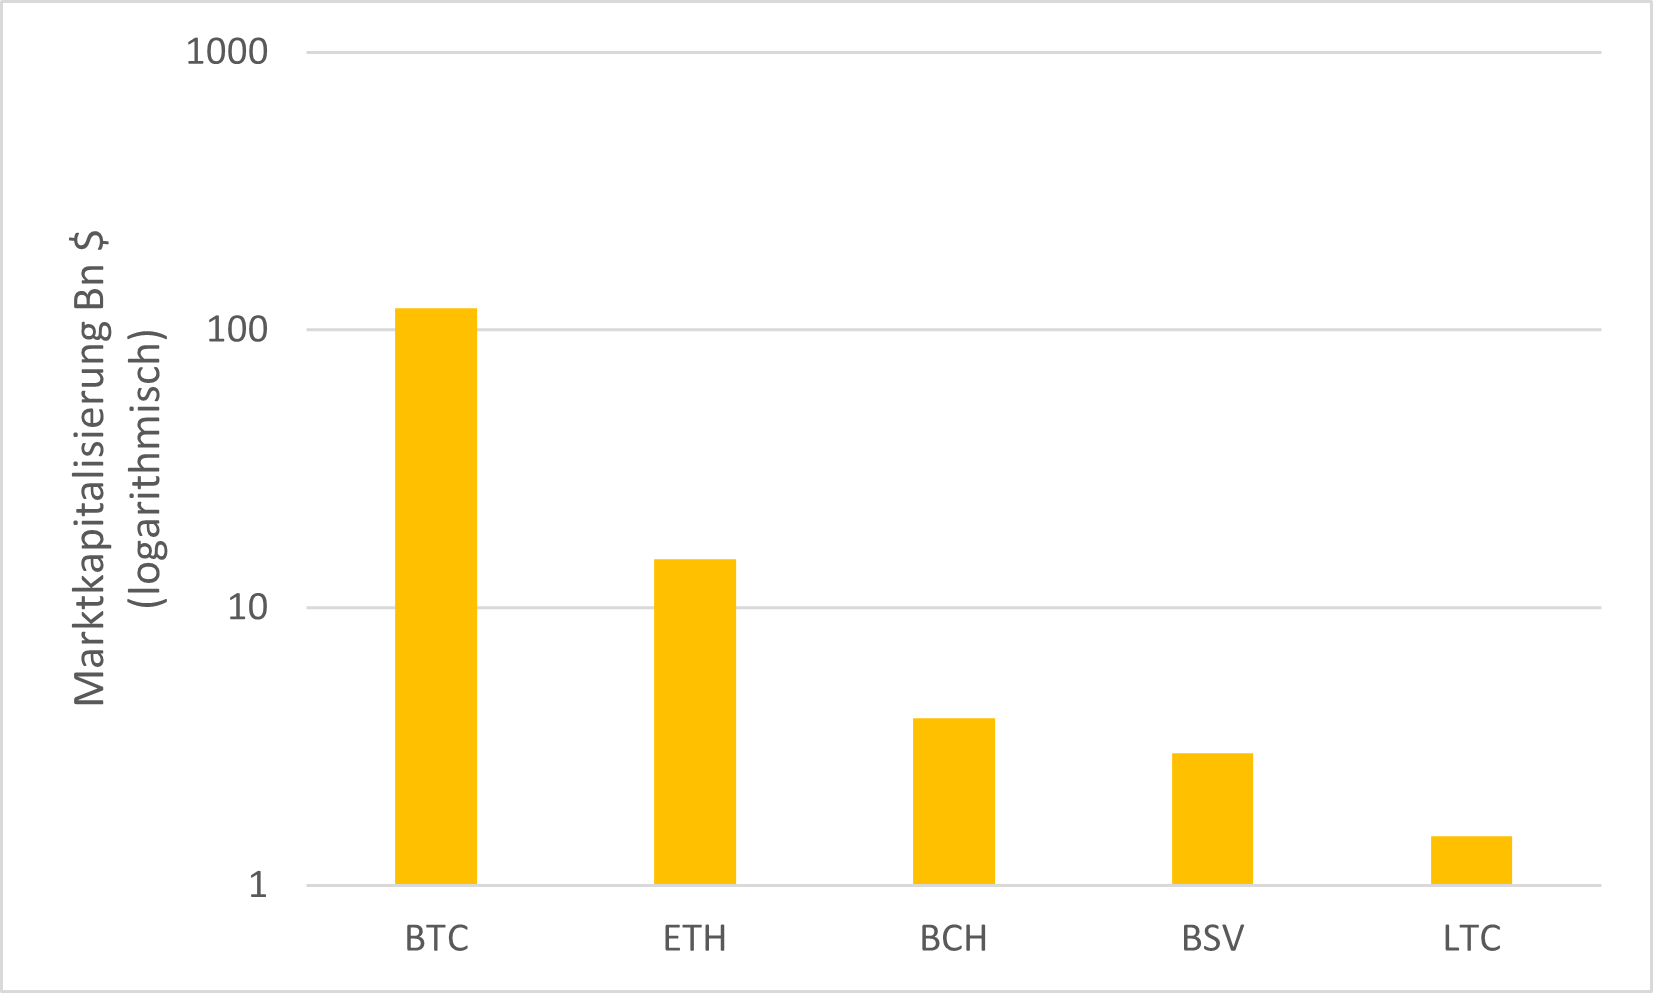
\includegraphics[width=.75\textwidth]{quellen/pow_mkp_2020.png}
    \caption{Marktanteil von PoW-Netzwerken 2020}
\end{figure}
\FloatBarrier